%!TEX root = ../../../thesis.tex

The amount of energy lost in a mechanical water meter has been estimated, as has the fraction of that energy which can be harnessed.
Now, the amount of energy required to operate an electronic water meter is sought.
This estimation will reveal how much further the cells built earlier would need to be improved to be viable.

\section{Microcontrollers}

  Central to the operation of an electronic water meter is the microcontroller (MCU).
  The primary function of the microcontroller is to read and log the amount of water consumed by the meter.
  The programme contained on the controller will also decide when to transmit that data and monitor energy usage.
  It is therefore a key component and is expected to consume the majority of energy.

  This chapter compares the power consumption and operational efficiencies of six low power MCUs deemed suitable for use in electronic metering applications.
  These microprocessors are low power, general purpose, 8-bit processors from Microchip, Atmel, and Freescale.
  Each of the microprocessors will have their energy consumption recorded while carrying out various functions over a range of supply voltages.
  Such measured functions are analogue-to-digital conversion, non-volatile memory writes, processing, and sleeping.


  \subsection{Selection of low power processors}

    \begin{sidewaystable}
      \begin{centering}
        \begin{tabular}{|l|l|l|l|l|l|l|l|}
        \cline{2-8}
        \multicolumn{1}{l|}{} & PIC16F1827  & PIC16F887  & PIC16F688  & PIC12F675  & ATtiny25V  & ATtiny13V  & MC9S08QG8 \tabularnewline
        \hline
        Vdd (min)  & 1.8  & 2.0  & 2.0V  & 2.0  & 1.8  & 1.8  & 1.8 \tabularnewline
        Vdd (max)  & 5.5  & 5.5  & 5.5V  & 5.5  & 5.5  & 5.5  & 3.6 \tabularnewline
        I (sleep)  & 30nA  & 50nA  & 50nA  & 1nA  & 100nA & <100nA & 450nA\tabularnewline
        CLOCK (min)  & 31kHz  & 31kHz & 31kHz & 31kHz & 16kHz & 16kHz & 1MHz \tabularnewline
        CLOCK (max)  & 32MHz  & 8MHz  & 8MHz  & 4MHz  & 16MHz & 9MHz  & 10MHz\tabularnewline
        EEPROM  & 256B  & 256B  & 256B  & 128B  & 128B  & 64B  & \dag{}\tabularnewline
        Serial  & USI  & USI  & USI  & --  & USI  & --  & USI \tabularnewline
        USART  & UART  & UART  & UART  & --  & --  & --  & -- \tabularnewline
        ADC  & 10bit  & 10bit & 10it  & 10bit & 10bit & 10bit & 10bit\tabularnewline
        \hline
        \end{tabular}
      \end{centering}

      \begin{centering}
      \dag Has 8,192 bytes of software programmable flash (16 pages of 512 bytes each).
      \end{centering}

      \begin{centering}
      \ddag Has 256 bytes of software programmable flash (4 pages of 64 bytes each).
      \end{centering}

      \caption{\label{tab:MCUfeaturecomparison} Feature comparison of benchmarked microprocessors.}
    \end{sidewaystable}

    The following processors were chosen from the three chosen manufacturers.
    \begin{itemize}
    \item Microchip PIC16F1827
    \item Microchip PIC16F688
    \item Microchip PIC12F675
    \item Atmel ATtiny25V
    \item Atmel ATtiny13V
    \item Freescale MC9S08QG8
    \end{itemize}
    A basic feature comparison of the MCU selection is shown in table \ref{tab:MCUfeaturecomparison}.





% \section{Power consumption}

% Each of the MCUs were programmed to carry out various tasks which
% were performed over their specified range of operating voltages and
% operating frequencies. While the chips where carrying out these tasks
% their power consumption was measured by an Agilent E5270B Precision
% Mainframe via a PC and a Tektronix MSO 4054 Oscilloscope for timing
% purposes. Details on how each of the tests where carried out, as well
% as raw data, can be found in appendix %\ref{Appendix:Measurements} .


  \subsection{Benchmarking power consumption}

    It is important to ensure that each processor is operated so as to minimise power consumption, which meant taking certain precautions.
    Spare pins were set as outputs and tied to Vdd with \SI{10}{\kilo\ohm} resistors.
    Unused peripherals were disabled including any watchdog timers and brownout detection circuitry.
    To allow more accurate sleep current measurements, the chips were placed in a chip carrier with \SI{10}{\kilo\ohm} resistors soldered between the general purpose pins and Vdd.
    The chip and carrier was washed in isopropyl alcohol and dried before being suspended by connections to the measurement device.
    This step minimises leakage current between the pins due to oils and dirt that may be transferred by touching or resting on a table.
    Measurements were carried out using the Agilent E5270B Precision Measurement Mainframe.
    This device has been used for most other measurement situations throughout this thesis for its high impedance inputs and measurement accuracy.


    \subsubsection{Sleep mode}


      \begin{figure}
        \centering
        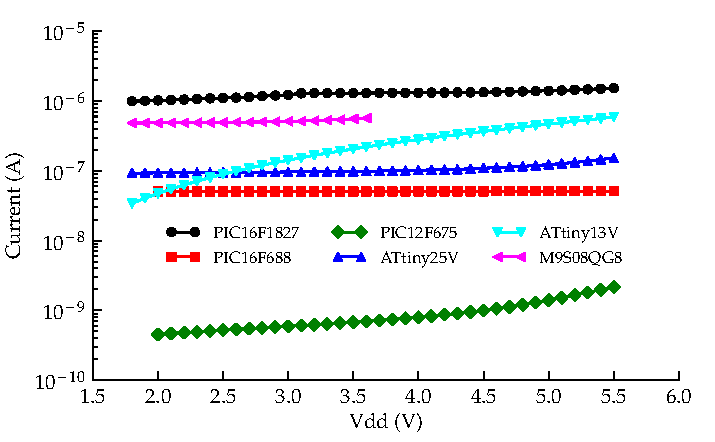
\includegraphics{content/pt1/03-EnergyRequirements/graphics/Graph_All_Sleeping_Current}
        \caption{\label{fig:All_Sleep_Current}Graph showing current consumed by MCUs in sleep mode versus supply voltage.}
      \end{figure}

      A microprocessor in sleep mode is essentially powered off, the difference being that volatile data is preserved.
      In order to consume as little power as possible an MCU should spend as much time in sleep mode as possible.
      The power consumption while sleep states will determine a large part of the water meters overall energy requirements.

      \Cref{fig:All_Sleep_Current} shows the amount of current consumed by each MCUs while in their deepest sleep states.
      Surprisingly, the PIC16F1827 consumes the most current in this state, almost one thousand times more than the specified sleep current of \SI{30}{\nano\ampere}\cite{PIC16F1827}.
      The Freescale MC9S08QG8 consumed energy at an average of 11\% higher than specified \cite{MC9S08QG8}.
      Both the Atmel ATtiny13V and ATtiny25V fell within their specification, \cite{AtmelATtiny13,AtmelATtiny25} respectively.
      The Microchip PIC12F675 fell within specification\cite{PIC12F675} and was clearly ahead in terms of minimum current draw during sleep.

      There appears to be a trade-off between the two Atmel processors in the way of minimum power consumption and minimum response to Vdd.
      The ATtiny13V required approximately 2.7 times less power than the ATtiny25V at 1.8V, but above 2.5V the ATtiny25V is more draws less current.

      As the PIC16F1827 was so far off its specified value, measurements were repeated numerous times using code written in both assembler and HI-TECH C.
      A total of five different processors were tried, all giving the same result.
      All steps outlined in the PIC16F1827's datasheet to reduce power consumption had been followed.


    \subsubsection*{Disclaimer on processing}


      Measuring the amount of power required to process information is complicated.
      The way each chip carries out processing operations internally can differ from one another, even though all produce the same result.

      \begin{table}
        \centering
        \begin{tabular}{r|c}
          & Instructions\\
          \hline
          PIC16F1827 & 53\\
          PIC16F688 & 35 \\
          PIC12F675 & 35 \\
          ATtiny25V & 120 \\
          ATtiny13V & 120 \\
          MC9S08QG8 & 145
        \end{tabular}
        \caption{\label{tab:Number-of-instructions}Instruction-set size for each tested microprocessor.}
      \end{table}


      \begin{algorithm}
        \begin{lstlisting}
        if (danger >= 5) flight();
        else fight();
        \end{lstlisting}
        \caption{\label{alg:Simple-C-code-representation}Simple C-code representation of a branch instruction.}
      \end{algorithm}


      To illustrate, algorithm \ref{alg:Simple-C-code-representation} shows a simplified programme.
      To determine  the programme's outcome the processor must first evaluate whether `danger' is greater than or equal to five.
      Then it will either branch to the function `fight' or continue on to execute the function `flight'.

      \begin{algorithm}
        \begin{lstlisting}
        load 5 into register 001
        load danger into register 002
        branch-if-greater-or-equal 001 002 flight_call
        call-subroutine fight
        jump-to continue
        [flight_call]
        call-subroutine flight
        [continue]
        \end{lstlisting}
        \caption{\label{alg:Psudo-machine-code1}Pseudo machine-code representation
        of a branch instruction.}
      \end{algorithm}

      \begin{algorithm}
        \begin{lstlisting}
        load danger into register 001
        subtract-from-register 001 5
        branch-if-minus 001 fight_call
        call-subroutine flight
        jump-to continue
        [fight_call]
        call-subroutine fight
        [continue]
        \end{lstlisting}
        \caption{\label{alg:Psudo-machine-code2}Pseudo machine-code representation of an alternative branch instruction.}
      \end{algorithm}


      Algorithms \ref{alg:Psudo-machine-code1} and \ref{alg:Psudo-machine-code2} demonstrate two different ways of implementing \ref{alg:Simple-C-code-representation} using pseudo machine-code.
      The decision of which to use is made by the compiler, which \emph{should} take the instructional efficiency of the specific MCU into account.
      This is an overly simplistic example, but it illustrates that there are multiple paths leading to the same result.
      Importantly, not all of those paths require the same amount of effort on the processor's behalf.
      This means that the compiler's ability to optimise code efficiently plays a role in determining the overall performance of the chip.
      This also means that the programmer should not be concerned with instructional efficiency as the compiler should transform C-code into machine code that best suits the target MCU.

      Another factor in processing efficiency comes down to the number of different instructions it is capable of.
      The list of instructions a processor is capable of is called its instruction set.
      Most 8-bit MCUs are based on reduced instruction set computing (RISC) architecture, as opposed to complex instruction set computing (CISC).
      When compared to a CISC based CPU, a RISC based chip is simpler and therefore usually cheaper to produce and simpler to program.
      However, ``Instruction traces from CISC machines consistently show that few of the available instructions are used in most computing environments''\cite{ComputerArch}, meaning that many of the extended operations in CISC designs are underutilised.
      Processors with smaller instruction sets are capable of achieving the more complex operations by chaining multiple instructions together.
      This means that processors with smaller instruction sets may take longer to execute certain instructions.
      Finally, the frequency of a microprocessor isn't necessarily the frequency at which it performs operations, although sometimes it is.
      For instance, the Atmel and Freescale microprocessors perform one instruction per clock cycle, whereas the Microchip processors perform one instruction every four clock cycles.


    \subsubsection{Processing}

      \begin{figure}
        \centering
        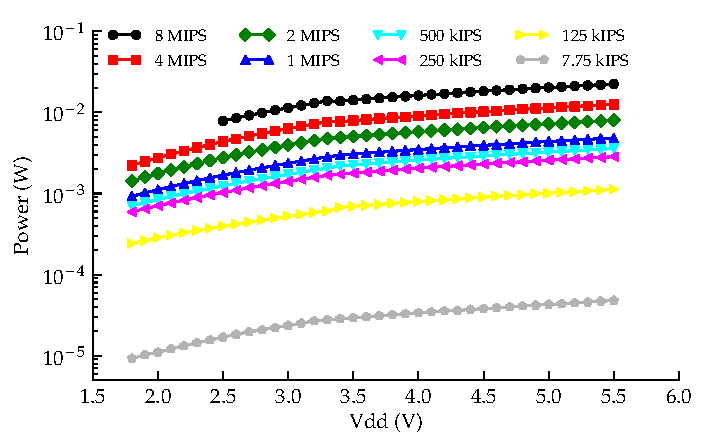
\includegraphics{content/pt1/03-EnergyRequirements/graphics/Graph_PIC16F1827_Clock_Power}
        \caption{\label{graph:CLK_POWER_16F1827}Graph showing power consumed by the PIC16F1827 while processing versus supply voltage.}
      \end{figure}

      \begin{figure}
        \centering
        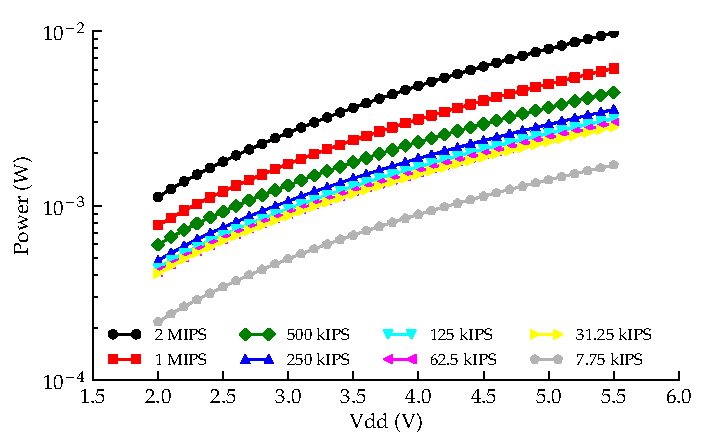
\includegraphics{content/pt1/03-EnergyRequirements/graphics/Graph_PIC16F688_Clock_Power}
        \caption{\label{graph:CLK_POWER_16F688}Graph showing power consumed by the PIC16F688 while processing versus supply voltage.}
      \end{figure}

      \begin{figure}
      \centering
        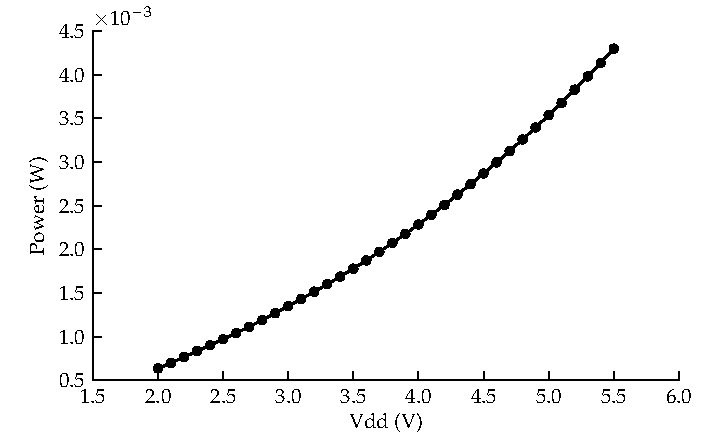
\includegraphics{content/pt1/03-EnergyRequirements/graphics/Graph_PIC12F675_Clock_Power}
        \caption{\label{graph:CLK_POWER_12F675-1}Graph showing power consumed by the PIC12F675 while processing versus supply voltage.}
      \end{figure}

      \begin{figure}
      \centering
        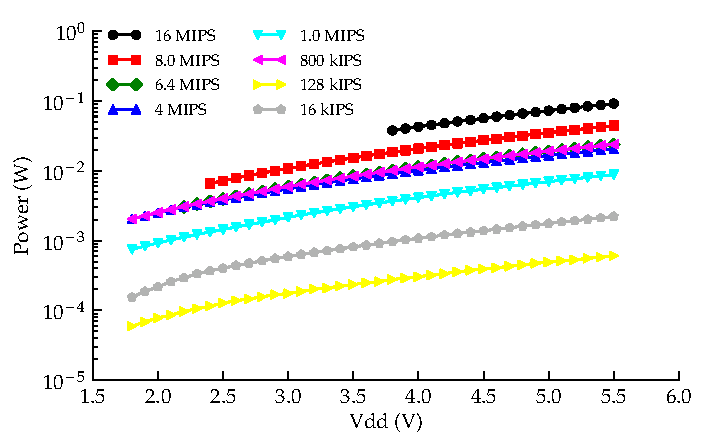
\includegraphics{content/pt1/03-EnergyRequirements/graphics/Graph_ATtiny25V_Clock_Power}
        \caption{\label{graph:CLK_POWER_ATtiny25V}Graph showing power consumed by the ATtiny25V while processing versus supply voltage.}
      \end{figure}

      \begin{figure}
        \centering
        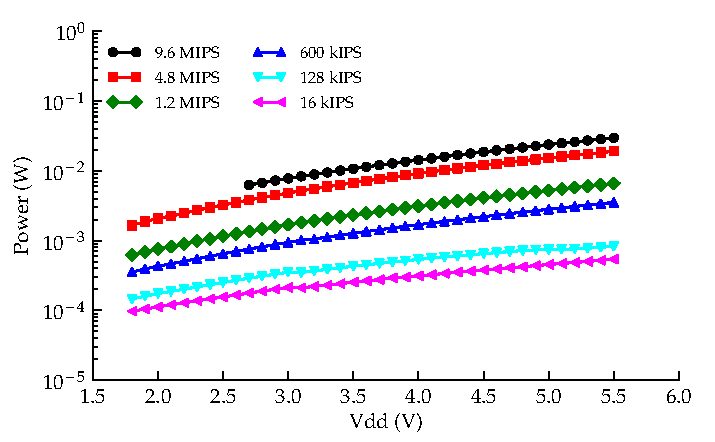
\includegraphics{content/pt1/03-EnergyRequirements/graphics/Graph_ATtiny13V_Clock_Power}
        \caption{\label{graph:CLK_POWER_ATtiny13V}Graph showing power consumed by the ATtiny13V while processing versus supply voltage.}
      \end{figure}

      \begin{figure}
        \centering
        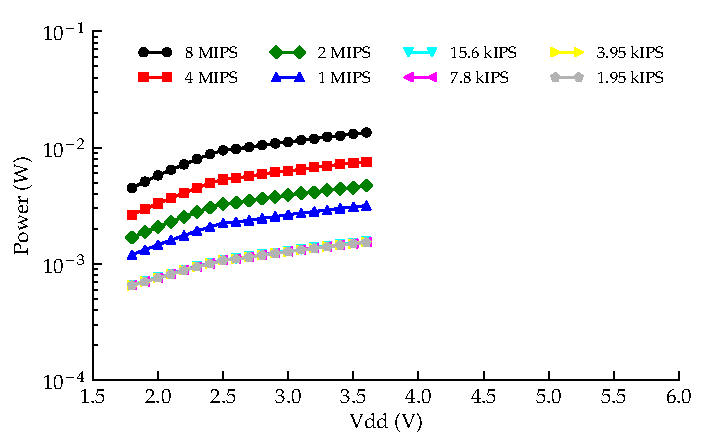
\includegraphics{content/pt1/03-EnergyRequirements/graphics/Graph_MC9S08QG8_Clock_Power}
        \caption{\label{graph:CLK_POWER_MC9S08QG8}Graph showing power consumed by the MC9S08QG8 while processing versus supply voltage.}
      \end{figure}

      Results in this section are expressed in terms of instructions per second (IPS).
      The Microchip PIC16F1827 displayed the lowest energy usage with \SI{10}{\micro\ampere} while clocking \SI{7.75}{\kilo IPS} (as shown in \cref{graph:CLK_POWER_16F1827}).
      Microchip MCUs complete one instruction every four clock cycles, so the \SI{7.75}{\kilo IPS} actually corresponds to a standard clock frequency of \SI{31}{\kilo\hertz}.

      % Edit checkpoint 2015-09-17 18:59

      \Cref{graph:CLK_POWER_16F688} shows that the PIC16F688 consumes less power than the PIC16F1827 at low voltages for the same instruction rates (except at 7.75kIPS).
      There appears to be a flatter response in power consumption with respect to Vdd in the PIC16F1827.
      Again, this appears to be a similar trade-off to what was mentioned earlier (in \cref{fig:All_Sleep_Current}) with the Atmel chips.

      The PIC12F675 (\cref{graph:CLK_POWER_12F675-1}) used approximately the same power as the PIC16F688 (\cref{graph:CLK_POWER_16F688}) for its \SI{1}{\mega IPS} trace.
      \Cref{graph:CLK_POWER_ATtiny25V,graph:CLK_POWER_ATtiny13V} show both Atmel MCUs having similar requirements.
      The MC9S08QG8, although being able to clock the slowest, performed very poorly at low frequencies.
      At \SI{1.95}{\kilo IPS} it consumed approximately the same amount of power as the Microchip MCUs operating at \SI{1}{\mega IPS}.

      Overall, the PIC16F1827 gives the widest range of power consumption options, with the ATtiny25V offering similar performance options.

    \subsubsection*{Joules of energy consumed per instruction cycle\label{sub:Joules-of-energy}}

      A convenient, and more insightful way to interpret the previous processing power consumption graphs is to calculate the energy spent per instruction performed.
      The energy cost of an instruction cycle can be calculated using equation \ref{eq:JPI calculation}.

      \begin{equation}
      E_{i}=\frac{I\times Vdd}{f_{i}}\label{eq:JPI calculation}
      \end{equation}
      where $E_{i}$ is the number of joules consumed per instruction, $I$ is the current draw, $Vdd$ is the input voltage and $f_{i}$ is the instruction frequency.

      Figure \ref{fig:Per-instruction-cycle} compares the most energy efficient operating conditions of each of the tested chips.
      What is most interesting about this graph is the high degree of overlap.
      Also, the greater efficiencies occur at high operating frequencies.
      A simple rule of thumb for selecting the most power efficient operating frequency based on these results is to choose the highest frequency where the MCU can operate over its full input voltage (Vdd) range.
      For comparison, figure \ref{fig:Per-instruction-ATtiny13V} shows the trade-off made when selecting a higher frequency, which is typical across the range of MCUs tested.

      \begin{figure}
      \begin{centering}
      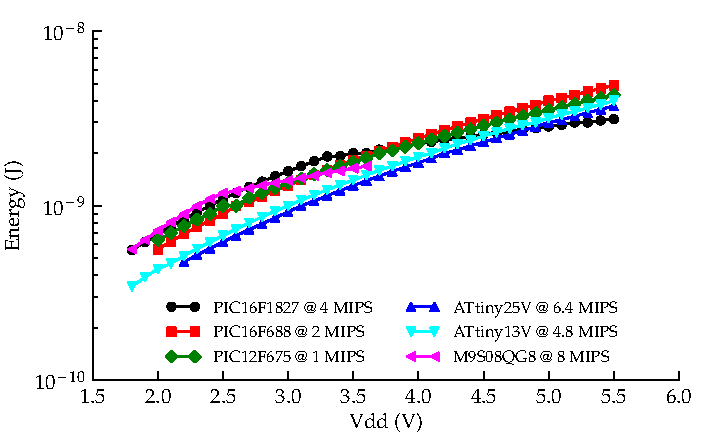
\includegraphics{content/pt1/03-EnergyRequirements/graphics/Graph_All_Clock_JPI}
      \par\end{centering}

      \protect\caption{\label{fig:Per-instruction-cycle}Graph showing instruction cycle energy consumption for each MCU versus supply voltage.}
      \end{figure}
      \begin{figure}
      \begin{centering}
      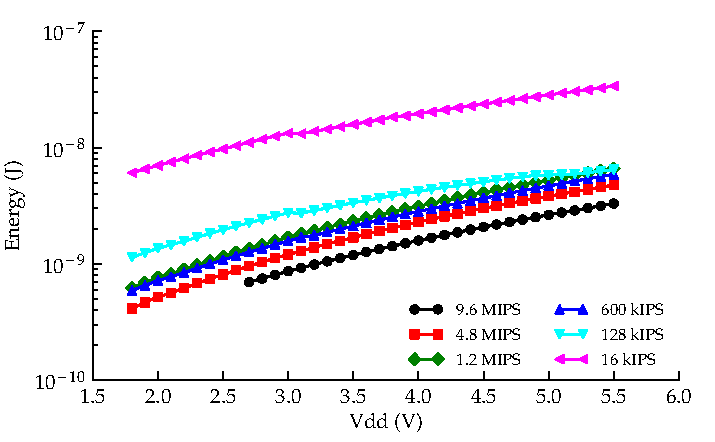
\includegraphics{content/pt1/03-EnergyRequirements/graphics/Graph_ATtiny13V_Clock_JPI}
      \par\end{centering}

      \protect\caption{\label{fig:Per-instruction-ATtiny13V}Graph showing instruction cycle energy consumption of the ATtiny13V versus supply voltage.}
      \end{figure}



    \subsubsection{Instruction efficiency}

      \begin{algorithm}
        \begin{lstlisting}
          unsigned short lfsr = 0xACE1u;
          unsigned period = 0;
          do {
            lfsr = (lfsr >> 1) ^ (-(lfsr & 1u) & 0xB400u);
            ++period;
          } while(lfsr != 0xACE1u);
        \end{lstlisting}
        \caption{\label{alg:Benchmarking-algorithm}Benchmarking algorithm}
      \end{algorithm}

      Calculating the amount of energy consumed per instruction only shows part of processor efficiency.
      The amount of processing done per instruction is not taken into account in such measurements.
      Some MCUs have extra instructions that are designed to help speed up code execution by combining commonly used groups of instructions.
      To shed light on instructional efficiency, the number of instructions each of the processors takes to complete a benchmark function is found.
      This will allow for a more accurate representation of execution efficiency.
      The function used to benchmark each of the processors is a linear feedback shift register based pseudo-random number generator \cite{Wikipedia2015}.
      It is well suited to an 8-bit microprocessor as it requires no complex math functions, uses little memory and has a well defined end.
      The code for this function is shown as \cref{alg:Benchmarking-algorithm}.
      It starts with a 16-bit number and runs it through the linear feedback register in a tight loop until the initial value of the 16-bit feedback register is produced again.
      This function steps through every possible combination of bits possible in a 16-bit number (except for 0 and 65535) in a pseudo-random order before exiting the loop.
      The function combines the exclusive-OR (XOR), bit shifting, bitwise AND, increment a value and numerical comparison operations in a tight loop.
      The benchmarking function was compiled and run on each of the MCUs operating at a range of supported frequencies.

      \begin{figure}
          \begin{centering}
              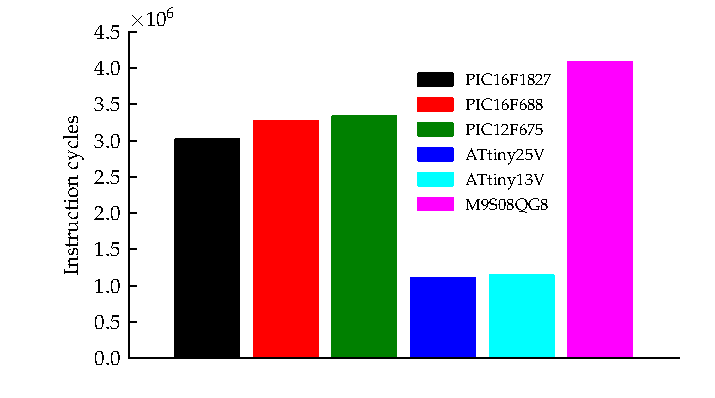
\includegraphics{content/pt1/03-EnergyRequirements/graphics/Graph_All_Clock_Benchmark}
          \end{centering}
          \protect\caption{\label{fig:GraphBar_All_Benchmark}Graph showing the number of instruction cycles taken to complete a benchmark routine for each MCU.}
      \end{figure}

      To determine the instructional efficiency, the code was set to toggle the state of a digital output pin.
      The toggle frequency of that pin was recorded using a Tektronix MSO 4054 oscilloscope.
      The number of instruction cycles each chip took to complete the benchmark was deduced by multiplying the time taken to complete the benchmark by the instruction cycle frequency.
      The results of the benchmark are shown in \cref{fig:GraphBar_All_Benchmark}.
      To calculate the number of instruction cycles taken by the Microchip family of processors, one quarter of the chip's operation frequency was used.
      This meant that the number of clock cycles consumed was four times higher.
      It is clear from \cref{fig:GraphBar_All_Benchmark} that the Atmel (ATtiny25V and ATtiny13V) microprocessors are by far the most efficient microprocessor in terms of executing code using a minimum number of instructions of the selection.
      The reason for this is most probably due to the larger instruction set and higher compiler optimisation.



    \subsubsection{Non-volatile memory}

      In order for a microprocessor to keep information about its current state and recorded data in the event of power loss it must write to non-volatile memory.
      Non-volatile memory is implemented as either electrically erasable and programmable read only memory (EEPROM) or Flash memory.
      Flash memory is similar to EEPROM with the exception that it must be erased in large blocks, or pages, before it can be written to.
      All of the tested MCUs have on-board EEPROM with the exception of the MC9S08QG8 which has flash memory instead.
      Table \ref{tab:MCUfeaturecomparison} shows the amount of non-volatile memory space available on each of the chips.

      \begin{figure}
        \centering
        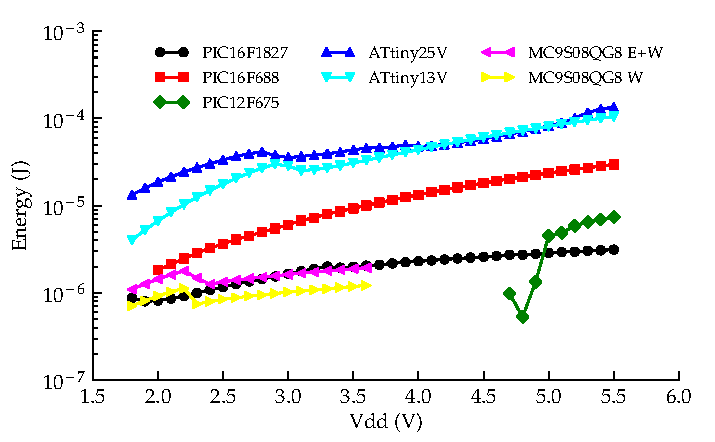
\includegraphics{content/pt1/03-EnergyRequirements/graphics/Graph_All_EEPROM_JPO}
        \caption{\label{fig:Energy-consumed-EEPROM}Graph showing energy consumed per non-volatile erase/write operation versus MCU supply voltage.}
      \end{figure}

      The energy consumption of each of the chips with EEPROM memory during a 1-byte write operation is shown as \cref{fig:Energy-consumed-EEPROM}.
      A curious situation arose with the PIC12F675 where its calculated energy consumption was negative when operated below \SI{4.7}{\volt}.
      It consumed \emph{less} current while performing write operations than running through the same code loop without performing writes.
      The measurement was repeated several times and produced the same result.
      Those data points were excluded from the plot as they do not represent the true energy cost of writing to EEPROM.
      It is likely that while writing to EEPROM other parts of this chip are disabled or put to sleep.

      In the case of the MC9S08QG8, which has Flash memory instead of EEPROM, the power consumption in the `E + W' trace was calculated as $1/512^{th}$ of consumed page erase energy consumption added to the energy cost of a single write operation.
      The trace labelled `W' (magenta) shows the energy cost for a single write operation.
      In order for the MC9S08QG8 to perform a write operation, the destination byte must have already been pre-erased at an earlier point in time.
      This may be useful for power harvesting since the energy expensive page erase operation, which consumes an average of \SI{302}{\micro\joule}, can be performed when available energy is plentiful.
      These results show that the Microchip and Freescale microprocessors are the most energy efficient when writing to non-volatile memory.



    \subsubsection{Analog-to-digital conversion}

      The operation of an electronic water meter may require that analogue-to-digital conversions are made.
      Measuring the amount of energy consumed per conversion was done in much the same way as the previous tests.
      Each of the chips had similar converters feature-wise.
      Results from the measurements are presented as \cref{fig:Energy-consumed-ADC}.

      \begin{figure}
        \centering
        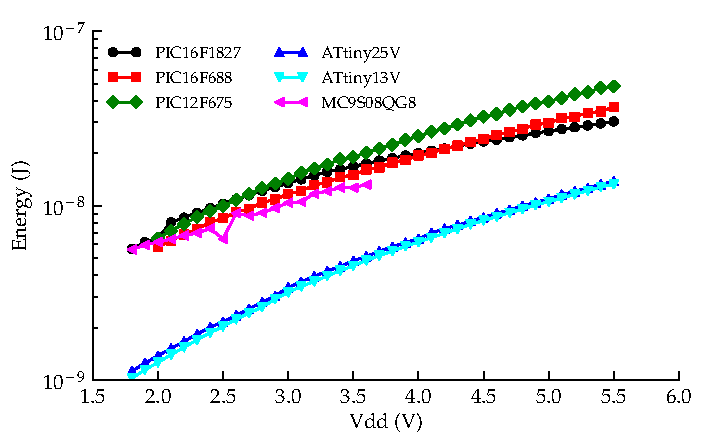
\includegraphics{content/pt1/03-EnergyRequirements/graphics/Graph_ALL_ADC_JPM}
        \caption{\label{fig:Energy-consumed-ADC}Graph showing the energy consumed per ADC measurement versus MCU supply voltage.}
      \end{figure}


  \section{Wireless Transmission}

    Because water meters are typically installed in remote areas where grid connection is unavailable, data must be collected via wireless interface.
    In Hamilton, a major utility provider has established a wireless mesh network between smart electricity meters installed in residential homes.
    That network utilises ZigBee wireless transceivers, making ZigBee an convenient choice for transmitting water metering data \cite{MalcolmSouness-WELNetworks2012}.
    Two types of wireless transmitters were chosen for energy measurement, a HOPE RF RFM12B transceiver and a Digi International Xbee Series 2 transceiver.
    The power consumption versus time during a wake, send one hundred and sixty bytes, and power down cycle was captured for both transceivers.
    By integrating the area under this curve the total energy consumed per transmission is found.
    The transmitters were kept \SI{1}{\meter} from their receivers with no obstructions between them.
    This represents ideal transmission conditions, something that our electronic water meter is very unlikely to encounter.
    The actual RF reception between a base station and installed meter will vary greatly between installations and weather conditions.
    For example, wet ground is likely to obstruct RF transmission due to the transmitter being shielded by a more conductive medium.
    Instead of trying to quantify the energy required in those situations, the best case was measured and an estimate of the worst case is estimated to be one hundred times larger.
    The transmit power can increase by a factor of 320 for the RFM module, however the transmit power only represents a proportion of total power usage.
    The modules must power up, start their internal oscillators, receive the data to be transmitted from the main processor and then transmit the data packets.
    I have crudely estimated that the difference between the lowest and the highest total power consumption, based on reception alone, will be a factor of 100.

    \begin{figure}
      \centering
      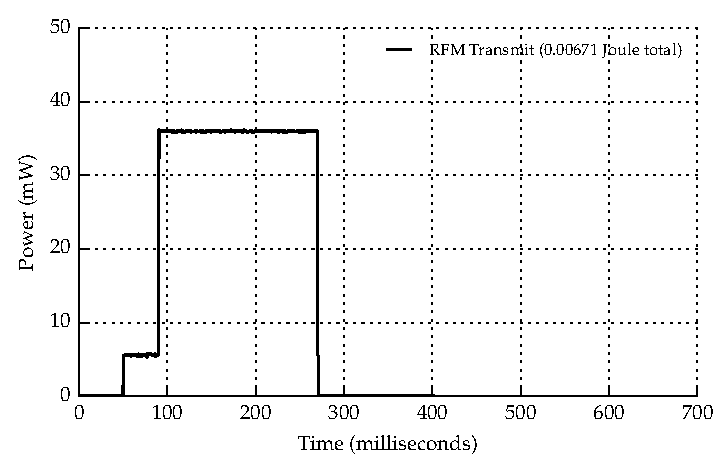
\includegraphics{content/pt1/03-EnergyRequirements/graphics/Graph_RFMPower.pdf}
      \caption{\label{fig:Energy-consumed-RFM12B}Graph of power draw from a HopeRF RFM12B transceiver module versus time during a power-up and transmit sequence.}
    \end{figure}

    \begin{figure}
      \centering
      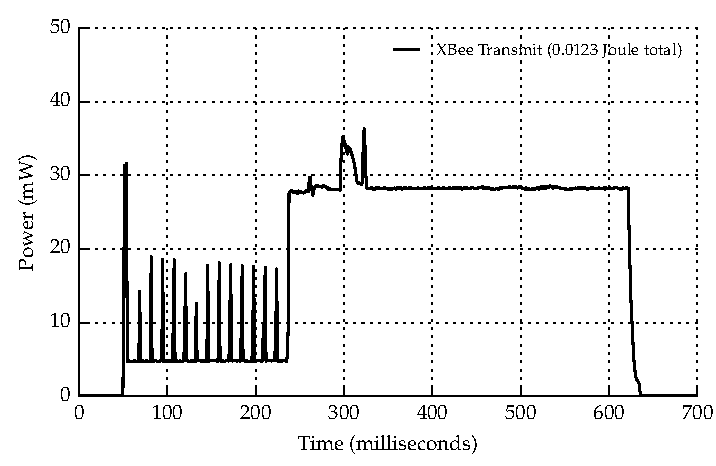
\includegraphics{content/pt1/03-EnergyRequirements/graphics/Graph_XbeePower.pdf}
      \caption{\label{fig:Energy-consumed-XBee}Graph of power draw from a Digi International Xbee Series 2 transceiver module versus time during a wake \& transmit sequence.}
    \end{figure}

    The RFM12B operates with a carrier frequency of \SI{433}{\mega\hertz}, a globally available and license-free frequency.
    It has been shown that frequencies in the \SI{300}--\SI{400}{\mega\hertz} range reduce the path loss in buried transmitter situations to a level that allows feasible communication~\cite{Li2007}.
    Additionally, \SI{433}{\mega\hertz} has the ability to penetrate concrete and water~\cite{Arsalan2012}.
    It has a maximum output power of \SI{5}{\decibel m} (\SI{3.2}{\milli\watt}) at this frequency.
    The Xbee has a maximum output power of \SI{0}{\decibel m} (\SI{1}{\milli\watt}) and operates at \SI{2.4}{\giga\hertz}.
    \Cref{fig:Energy-consumed-RFM12B,fig:Energy-consumed-XBee} show the captured power consumption during the tests.
    The RFM12B used about half as much energy sending the same data as the Xbee.
    Combined with its favourable communication frequency, the RFM12B is a sensible choice for the electronic water meter.
    In total the RFM consumed \SI{6.71}{\milli\joule} and the Xbee consumed \SI{12.3}{\milli\joule}.
    Adjusting these figures for the worst case (multiplying by one hundred) gives \SI{671}{\milli\joule} for the RFM12B and \SI{1.23}{\joule} for the Xbee.

  \section{Final Estimate of Energy Requirements}

    A crude estimation of an electronic water meter's microprocessor event loop is as follows.
    \begin{enumerate}
      \item Sleep for 1 second
      \item Execute 1000 instructions
      \item Make 2 analogue conversions
      \item Write 2 bytes to non-volatile memory
    \end{enumerate}
    This would allow the microprocessor to watch the display of a mechanical water meter and store the readings.
    This loop would occupy approximately one second, so it will occur 86400 times per day.
    Every so often the collected data would need to be transmitted, a potentially costly exercise in terms of energy usage.
    On top of the previously stated event loop is a data transmission loop which would execute every six hours.
    \begin{enumerate}
      \item Execute 1000000 instructions (Data compression)
      \item Power up and transmit 160 bytes of using RF transceiver
      \item Write 10 bytes to non-volatile memory
    \end{enumerate}

    \begin{table}
      \centering
      \begin{tabular}{|l|l|l|l|}
        \hline
        Mode & Count & Unit & Energy \\ \hline
        Sleep & 1 & seconds & \SI{97.4}{\nano\joule} \\
        Processing & 1000 & instructions & \SI{1.14}{\micro\joule} \\
        ADC & 2 & conversions & \SI{2.56}{\nano\joule} \\
        EEPROM & 2 & bytes & \SI{79.0}{\micro\joule} \\ \hline \hline
        &&Total (per day) & \SI{6.93}{\joule} \\ \hline
      \end{tabular}
      \caption{\label{tab:EnergyBudget-EventLoop} Estimated daily energy expenditure for basic processing functionality}
    \end{table}

    \begin{table}
      \centering
      \begin{tabular}{|l|l|l|l|}
        \hline
        Mode & Count & Unit & Energy \\ \hline
        Processing & 1000000 & instructions & \SI{1.14}{\milli\joule} \\
        Transmit & 160 & bytes & \SI{1.23}{\joule} \\
        EEPROM & 10 & bytes & \SI{394}{\micro\joule} \\ \hline \hline
        &&Total (per day) & \SI{4.93}{\joule} \\ \hline
      \end{tabular}
      \caption{\label{tab:EnergyBudget-Transmission}Estimated daily energy expenditure required to transmit 160 characters every six hours}
    \end{table}

    \Cref{tab:EnergyBudget-EventLoop,tab:EnergyBudget-Transmission} combine the measurements and estimates from the previous sections with the event loop estimation.
    They show that approximately \SI{12}{\joule} would be consumed per day by an electronic water meter.
    It was shown in \cref{sect:part1-WirelessWaterMeter-QuantifyingHarvestableEnergy} that \SI{280}{\joule} of energy is already dissipated in a mechanical water meter per day.
    This equates to a conversion efficiency of \SI{4.28}{\percent}, which would be the minimum efficiency required to run the meter continuously.

    % Edit checkpoint 2015-09-17 19:35